\section{Theoretical framework}

\subsection{Graph theory}
This section contains definitions, notation and concepts related to Graph Theory according
to \cite{graph_theory:2010}.

\subsubsection{Simple graphs}
A \textbf{simple graph} \textit{G} consists of a non-empty finite set \textit{V(G)} of elements called \textbf{vertices}
(or \textbf{nodes}), and a finite set \textit{E(G)} of distinct unordered pairs of distinct elements of \textit{V(G)}
called \textbf{edges}. We call \textit{V(G)} the \textbf{vertices set} and \textit{E(G)} the \textbf{edge set} of G.
An edge $\{\textit{v}, \textit{w}\}$ is said to \textbf{join} the vertices v and w, and is usually abbreviated to vw. For example, Figure~\ref{fig:simple_graph} represents the simple graph G whose vertex set \textit{V(G)} is $\{\textit{u}, \textit{v}, \textit{w}, \textit{z}\}$, and whose
edge set \textit{E(G)} consists of the edges \textit{uv}, \textit{uw}, \textit{vw} and \textit{wz}. 

\begin{figure}[H]
    \centering
    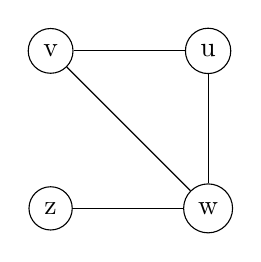
\begin{tikzpicture}
      % Disegno dei nodi
      \node[circle, draw] (v) at (0,0) {v};
      \node[circle, draw] (u) at (2,0) {u};
      \node[circle, draw] (w) at (2,-2) {w};
      \node[circle, draw] (z) at (0,-2) {z};
      
      % Disegno degli archi
      \draw (u) -- (v);
      \draw (u) -- (w);
      \draw (v) -- (w);
      \draw (w) -- (z);
    \end{tikzpicture}
    \caption{}
    \label{fig:simple_graph}
\end{figure}

\subsubsection{Adjacency}
We say that two vertices \textit{v} and \textit{w} of a graph \textit{G} are \textbf{adjacent} if there is an edge \textit{vw} joining them, and the vertices \textit{v} and \textit{w} are then \textbf{incident} with such an edge.
Similarly, two distinct edges \textit{e} and \textit{f} are \textbf{adjacent} if they have a vertex in common (see Figure \ref{fig:adiacency}).

\begin{figure}[H]
    \centering
    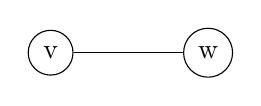
\begin{tikzpicture}
      % Primo grafo
      \node[circle, draw] (v) at (0,0) {v};
      \node[circle, draw] (w) at (2,0) {w};
      \draw (v) -- (w);
    \end{tikzpicture}
    \quad % Spazio tra i grafi
    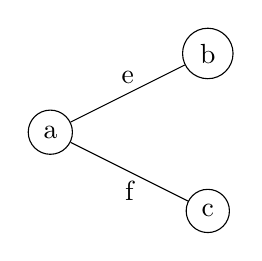
\begin{tikzpicture}
      % Secondo grafo
      \node[circle, draw] (a) at (0,0) {a};
      \node[circle, draw] (b) at (2,1) {b};
      \node[circle, draw] (c) at (2,-1) {c};
      \draw (a) -- node[above] {e} (b);
      \draw (a) -- node[below] {f} (c);
    \end{tikzpicture}
    \caption{Adjacent vertices and adjacent edges}
    \label{fig:adiacency}
\end{figure}

\subsubsection{Matrix representations}
Although it is convenient to represent a graph by a diagram of points joined by lines,
such a representation may be unsuitable if we wish to store a large graph in a computer.
One way of storing a simple graph is involve matrices. \\
Let's consider a graph \textit{G} with \textit{n} vertices and \textit{m} edges. \\
An \textbf{adjacency matrix A} is the $n \times n$ matrix whose \textit{ij}-th entry is the number of edges joining vertex \textit{i} and vertex \textit{j}. \\
If, in addition, the edges are labelled $\{1, 2, \dots, m\}$, its \textbf{incidence matrix M} is the $n \times m$ matrix whose \textit{ij}-th entry is 1 if vertex \textit{i} is incident to edge \textit{j}, and 0 otherwise. \\
An example of this is given in Figure \ref{fig:matrix_representations}.

\begin{figure}[H]
    \centering
    \begin{minipage}{0.5\textwidth}
        \centering
        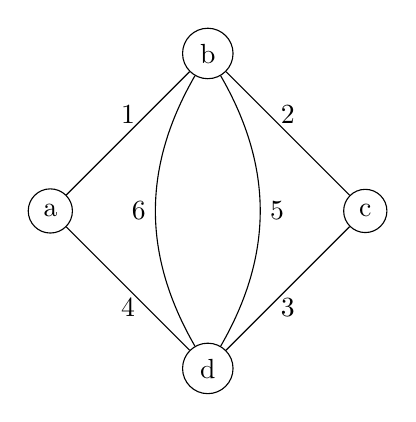
\begin{tikzpicture}
            % Nodi
            \node[circle, draw] (a) at (0,0) {a};
            \node[circle, draw] (b) at (2,2) {b};
            \node[circle, draw] (c) at (4,0) {c};
            \node[circle, draw] (d) at (2,-2) {d};
          
            % Archi
            \draw (a) edge node[pos=0.5, below] {4} (d);
            \draw (a) edge node[pos=0.5, above] {1} (b);
            \draw (b) edge[bend left] node[pos=0.5, right] {5} (d);
            \draw (b) edge[bend right] node[pos=0.5, left] {6} (d);
            \draw (b) edge node[pos=0.5, above] {2} (c);
            \draw (c) edge node[pos=0.5, below] {3} (d);
        \end{tikzpicture}
    \end{minipage}%
    \begin{minipage}{0.5\textwidth}
        \[
        A = \begin{bmatrix}
        0 & 1 & 0 & 1 \\
        1 & 0 & 1 & 2 \\
        0 & 1 & 0 & 1 \\
        1 & 2 & 1 & 0
        \end{bmatrix}
        \]
        
        \[
        M = \begin{bmatrix}
        1 & 0 & 0 & 1 & 0 & 0 \\
        1 & 1 & 0 & 0 & 1 & 1 \\
        0 & 1 & 1 & 0 & 0 & 0 \\
        0 & 0 & 1 & 1 & 1 & 1
        \end{bmatrix}
        \]
    \end{minipage}
    \caption{Graph \textit{G} with its adjacency and incidence matrices}
    \label{fig:matrix_representations}
\end{figure}


\subsubsection{Complete graphs}
A simple graph in which each pair of distinct vertices are adjacent is a \textbf{complete
graph}. \\
Here in Figure \ref{fig:complete_4} and in Figure \ref{fig:complete_5}, two examples of complete graphs.


\begin{figure}[H]
    \centering
    \begin{minipage}{0.45\textwidth}
        \centering
        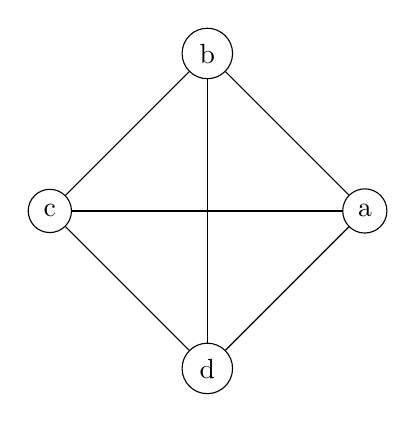
\begin{tikzpicture}
            % Grafo con 4 nodi
            \foreach \nodename/\nodeposition in {a/0, b/90, c/180, d/270}
                \node[circle, draw] (\nodename) at (\nodeposition:2) {\nodename};
            
            \foreach \startnode/\endnode in {a/b, a/c, a/d, b/c, b/d, c/d}
                \draw (\startnode) -- (\endnode);
        \end{tikzpicture}
        \caption{Complete graph with 4 vertices}
        \label{fig:complete_4}
    \end{minipage}%
    \hfill
    \begin{minipage}{0.45\textwidth}
        \centering
        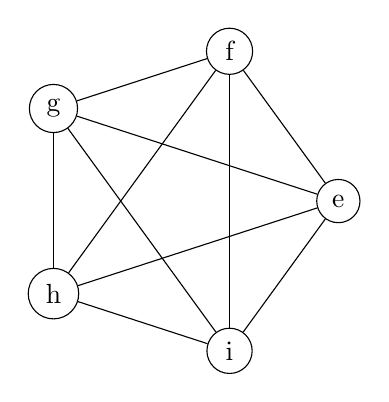
\begin{tikzpicture}
            % Grafo con 5 nodi
            \foreach \nodename/\nodeposition in {e/0, f/72, g/144, h/216, i/288}
                \node[circle, draw] (\nodename) at (\nodeposition:2) {\nodename};
            
            \foreach \startnode/\endnode in {e/f, e/g, e/h, e/i, f/g, f/h, f/i, g/h, g/i, h/i}
                \draw (\startnode) -- (\endnode);
        \end{tikzpicture}
        \caption{Complete graph with 5 vertices}
        \label{fig:complete_5}
    \end{minipage}
\end{figure}

\subsubsection{Bipartite graphs}
If the vertex set of a graph \textit{G} can be split into two disjoint sets \textit{A} and \textit{B} so that each
edge of \textit{G} joins a vertex of \textit{A} and a vertex of \textit{b}, then \textit{G} is a \textbf{bipartite graph}. \\
Alternatively, a bipartite graph is one whose vertices can be coloured black and white in such a way that each edge joins a black vertex (in \textit{A}) and a white vertex (in \textit{B}). \\
Figure \ref{fig:bipartite} is an example of bipartite graph.

\begin{figure}[H]
    \centering
    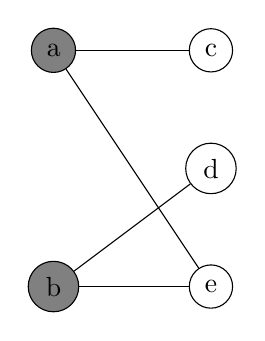
\begin{tikzpicture}[every node/.style={circle, draw, minimum size=0.2cm}]
        % Livello superiore
        \node (A) at (3,0) [fill=black!50] {a};
        \node (B) at (3,-3) [fill=black!50] {b};
        
        % Livello inferiore
        \node (C) at (5,0) [fill=white] {c};
        \node (D) at (5,-1.5) [fill=white] {d};
        \node (E) at (5,-3) [fill=white] {e};
        
        % Collegamenti
        \draw (A) -- (C);
        \draw (A) -- (E);
        \draw (B) -- (D);
        \draw (B) -- (E);
    \end{tikzpicture}
    \caption{}
    \label{fig:bipartite}
\end{figure}



\subsubsection{Bipartite graphs with matching}
A \textbf{bipartite graph with matching} is a bipartite graph in which there is a set of edges selected in such a way that no node is shared among the edges of the matching.
In other words, each node is involved in at most one edge of the matching. \\
This means that if the number of vertices in \textit{A} and \textit{B} is different, at least one vertex will have no connection to another vertex (see Figure \ref{fig:match_1}). \\
If there is the same number of vertices in both \textit{A} and \textit{B}, every vertex is connected to another vertex (see Figure \ref{fig:match_2}). \\
 
\begin{figure}[H]
    \centering
    \begin{minipage}{0.45\textwidth}
        \centering
        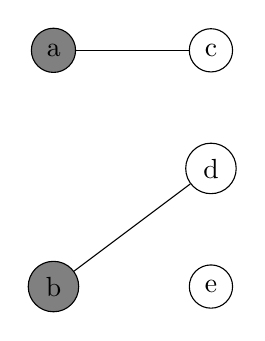
\begin{tikzpicture}[every node/.style={circle, draw, minimum size=0.2cm}]
            % Livello superiore
            \node (A) at (3,0) [fill=black!50] {a};
            \node (B) at (3,-3) [fill=black!50] {b};

            % Livello inferiore
            \node (C) at (5,0) [fill=white] {c};
            \node (D) at (5,-1.5) [fill=white] {d};
            \node (E) at (5,-3) [fill=white] {e};

            % Collegamenti
            \draw (A) -- (C);
            \draw (B) -- (D);
        \end{tikzpicture}
        \caption{}
        \label{fig:match_1}
    \end{minipage}
    \hfill
    \begin{minipage}{0.45\textwidth}
        \centering
        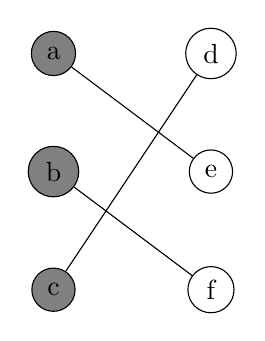
\begin{tikzpicture}[every node/.style={circle, draw, minimum size=0.2cm}]
            % Livello superiore
            \node (A) at (3,0) [fill=black!50] {a};
            \node (B) at (3,-1.5) [fill=black!50] {b};
            \node (C) at (3,-3) [fill=black!50] {c};

            % Livello inferiore
            \node (D) at (5,0) [fill=white] {d};
            \node (E) at (5,-1.5) [fill=white] {e};
            \node (F) at (5,-3) [fill=white] {f};

            % Collegamenti
            \draw (A) -- (E);
            \draw (B) -- (F);
            \draw (C) -- (D);
        \end{tikzpicture}
        \caption{}
        \label{fig:match_2}
    \end{minipage}
\end{figure}